\documentclass[a4paper, twocolumn]{article}
\usepackage[utf8]{inputenc}
\usepackage[T1]{fontenc}
\usepackage{lmodern}
\usepackage{hyperref}  % \href \url
\usepackage{physics}  % \dd{} \pdv{} \qty
\usepackage{graphicx}  % Inserting images.
\usepackage{siunitx}  % \si \SI
\usepackage{float}  % Allows for H float placement.
\usepackage{parskip}  % Separates paragraphs with vertical space.
\usepackage[margin=0.6cm]{geometry}
\usepackage{fancyvrb}

\begin{document}
\title{STK9900 -- Assignment 1}
\author{
    \begin{tabular}{r l}
        Jonas Gahr Sturtzel Lunde & (\texttt{jonassl})
    \end{tabular}}
% \date{}    % if commented out, the date is set to the current date
\maketitle

\section*{Problem 1}
\subsection*{a)}
We want to study the relationship between the observed amount of NO2 in the air, compared to a series of possible causes. First, we look at the relationship between the variables log.no2 and log.cars, plotted in figure \ref{fig:no2_cars_vs_no2}. There is definitively some positive correlation between the two quantities, although there is also a lot of deviations in the NO2 values not explained by log.cars.

A summary printout of the two observables gives the following:
\begin{Verbatim}[fontsize=\small]
> summary(data$log.cars)
Min. 1st Qu.  Median    Mean 3rd Qu.    Max. 
4.127   6.176   7.425   6.973   7.793   8.349 
> summary(data$log.no2)
Min. 1st Qu.  Median    Mean 3rd Qu.    Max. 
1.224   3.214   3.848   3.698   4.217   6.395 
\end{Verbatim}
As was already somewhat evident from the figure, log.cars is negatively skewed (has a tail in the negative direction), which is indicated by the fact that the mean of the data is noticably is lower than the median, while log.no2 is more symmetric.

\begin{figure}
    \centering
    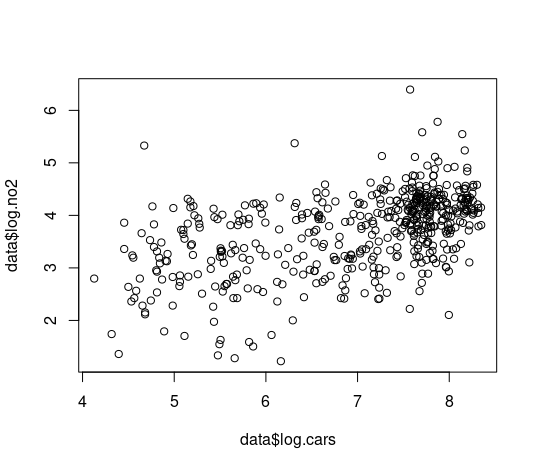
\includegraphics[width=0.8\linewidth]{figures/no2_cars_vs_no2.png}
    \caption{Scatter plot showing relation between the log amount of NO2 recorded versus the log amount of cars passing each hour.}
    \label{fig:no2_cars_vs_no2}
\end{figure}


\subsection*{b)}
A linear fit of log.no2 with log.cars as a predictor is plotted in figure \ref{fig:no2_cars_vs_no2_linfit}. As we noted, there seems to be a positive correlation between the two quantities, although the spread is large. The linear fit produced the following results:
\begin{Verbatim}[fontsize=\small]
 Estimate Std. Error t value Pr(>|t|)    
 (Intercept)  1.23310    0.18755   6.575 1.23e-10 ***
 log_cars     0.35353    0.02657  13.303  < 2e-16 ***
 Multiple R-squared: 0.2622,  Adjusted R-squared: 0.2607 
\end{Verbatim}
We see that the best fit is a positive slope of around 0.35, and an intercept of 1.23. As the intercept is far outside our oberved range, it should be ignored. The slope is statistically significantly different from zero, with a P-value numerically equivalent to zero ($<2\times 10^{-16}$). We also have $R^2 = 1 - \frac{\mathrm{RSS}}{\mathrm{TSS}} = 0.2622$, where RSS is the residual sum of squares, and TSS is the total sum of squares. The $R^2$ value tells us how large portion of the variance in log.no2 can be explained by our model alone (linear fit of log.cars). In other words, while we are confident that there is a relation between the two quantities, log.cars alone do not explain most of the behavior of log.no2. This is in line with what we visually observe from our figures.

\begin{figure}
    \centering
    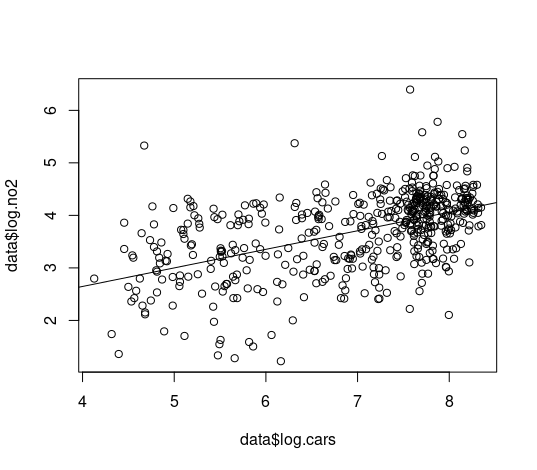
\includegraphics[width=0.8\linewidth]{figures/no2_cars_vs_no2_linfit.png}
    \caption{Linear fit of log.cars versus log.no2 plotted as a line over the scatter plot of the two observables.}
    \label{fig:no2_cars_vs_no2_linfit}
\end{figure}


\subsection*{c)}
Although we see a positive correlation between our two quantities, this doesn't mean that a linear model is the ideal fit. In order to assess our model choice, we should look at the residuals of our fit. In the case of a perfect model fit, the residuals should be normally distributed around 0. Figure \ref{fig:no2_residuals_plot} shows the residuals of our linear fit. There doesn't seem to be any obvious biases in the residuals, but we should not rely simply on visual inspection. Figure \ref{fig:no2_residuals_hist} shows a histogram of the residuals. The results look very promising, and the residuals seem to be very close to normally ditributed around 0. Finally, figure \ref{fig:no2_residuals_QQ} shows a QQ plot of the residuals. Such a plot follows a straight line (shown in the figure) in the case of a perfect guassian distribution. We see a slight but consistent deviation from this line. The S-shape indicates a slighly \textit{heavy-tailed} distribution, especially on the lower end, which fits well with a visual inspection of the histogram. The deviation in small, and overall the plots indicate that our linear model is a good choice.

\begin{figure}[h!]
    \centering
    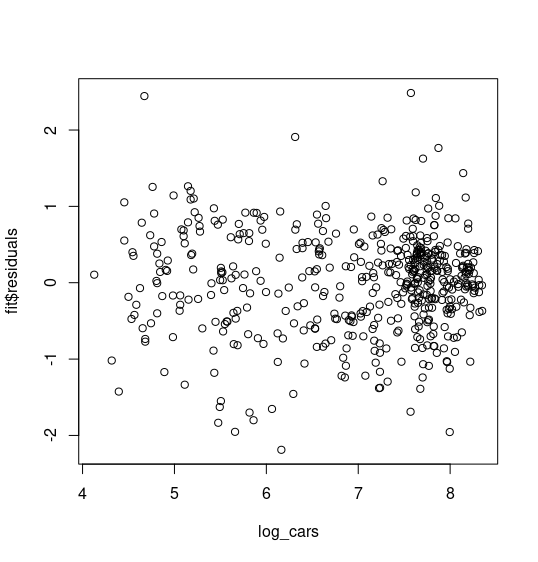
\includegraphics[width=0.7\linewidth]{figures/no2_residuals_plot.png}
    \caption{Scatter plot showing the residuals of the linear fit of log.cars to log.no2.}
    \label{fig:no2_residuals_plot}
\end{figure}

\begin{figure}[h!]
    \centering
    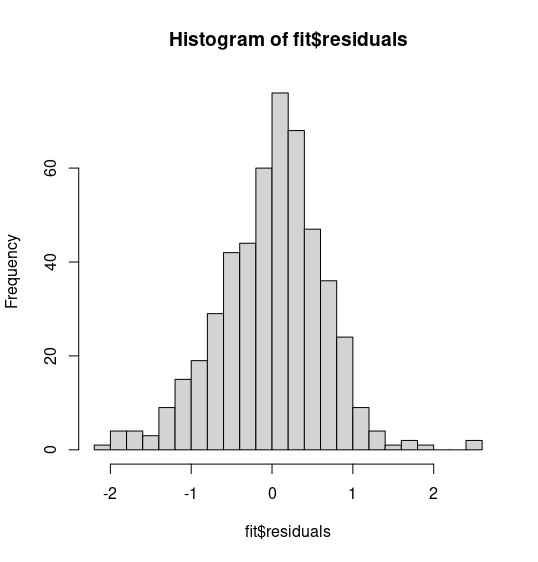
\includegraphics[width=0.7\linewidth]{figures/no2_residuals_hist.png}
    \caption{Histogram of the same residuals presented in figure \ref{fig:no2_residuals_plot}.}
    \label{fig:no2_residuals_hist}
\end{figure}

\begin{figure}[h!]
    \centering
    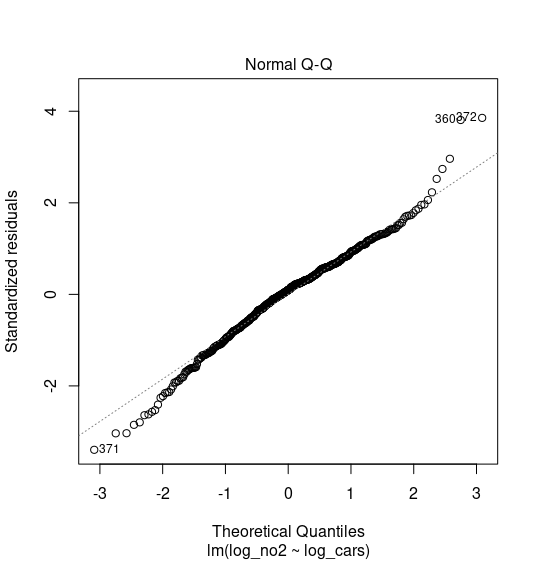
\includegraphics[width=0.7\linewidth]{figures/no2_residuals_QQ.png}
    \caption{QQ plot of the residuals presented in figure \ref{fig:no2_residuals_plot}. Normally distributed residuals (which is desirable) produce a straight line.}
    \label{fig:no2_residuals_QQ}
\end{figure}


\subsection*{d)}
We use the adjusted $R^2$ (which we'll simply refer to as $R^2$) to evaluate the quality of our models. The adjusted $R^2$ is a modification of the usual $R^2 = 1 - \frac{\mathrm{RSS}}{\mathrm{TSS}}$, which takes into account the number of independent variables in the fit in such a way that the adjusted $R^2$ value only increases if the addition of a new predictor increases the $R^2$ value more than could be expected from random chance. The ordinary $R^2$ value, meanwhile, is simply incapable of decreasing for additional predictors.

Below is a summary of a linear fit for NO2 as function of the 4 other observables.
\begin{Verbatim}[fontsize=\small]
    Estimate Std. Error t value Pr(>|t|)    
(Intercept)  1.152131   0.175045   6.582 1.19e-10 ***
log.cars     0.456974   0.028411  16.084  < 2e-16 ***
temp        -0.026855   0.003905  -6.877 1.85e-11 ***
wind.speed  -0.149334   0.014076 -10.609  < 2e-16 ***
hour.of.day -0.013025   0.004452  -2.926   0.0036 ** 
---
Residual standard error: 0.5508 on 495 degrees of freedom
Multiple R-squared: 0.4658,  Adjusted R-squared: 0.4615 
\end{Verbatim}
\subsubsection*{Number of cars}
The by far most siginficant correlation is with the log number of cars, at a t-value of $|t| = 16.084$. We seem to already have a pretty decent fit, but we can always try to improve it. The predictor is already log-transformed, but if we undo the logarithm, we can try a couple of other things. Simply using the linear number of cars as a predictor works very badly. We therefore look for a transformation which is similar to the logarithm. We try doing the square root, which improves the $R^2$ score from 0.4615 to 0.4645, and then the cube root, which improves it further to 0.4679. Further roots do not improve the results.


\subsubsection*{Wind speed}
The second strongest correlation is with the wind speed, at $|t| = 10.609$. The relation is plotted in figure \ref{fig:no2_windspeed_vs_no2}. We see that there is a negative correlation, which is perhaps slightly convex. The wind speed is also unevenly distributed, with more speeds closer to zero. We try to repeat the fit with the logarithmic wind speed, which produces a sligtly improved result, with $|t| = 11.726$, and an adjusted R squared of $0.4865$ (up from 0.4679).

\begin{figure}[h!]
    \centering
    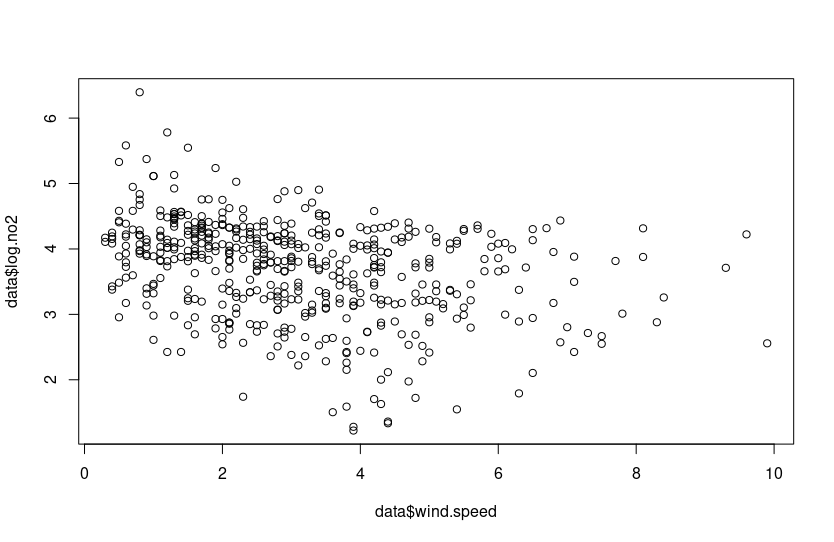
\includegraphics[width=0.7\linewidth]{figures/no2_windspeed_vs_no2.png}
    \caption{Scatter plot of log NO2 as fuction of wind speed.}
    \label{fig:no2_windspeed_vs_no2}
\end{figure}


\subsubsection*{Tempearture}
The third strongest correlation is with the temperature, at $|t| = 6.877$. This relation is plotted in figure \ref{fig:no2_temp_vs_no2}. We see a slighly negative correlation. As the zero-point of celsius temperature is arbritrary, we first convert the temperature to Kelvin for transformations. We try using the exponential, logarithmic, square root, and inverse of the Kelvin temperature as a predictior. They all produce very similar results, and although some have a slightly higher $R^2$-value than the linear temperature (0.4834 vs 0.4833), we consider it non-significant. The transformation $\sqrt{\mathrm{temp} + 20}$ improved the $R^2$ from 0.4863 to 0.4873. However, this is an unfomfortable model for other reasons: temperatures below -20 degrees produce non-real solutions.

\begin{figure}[h!]
    \centering
    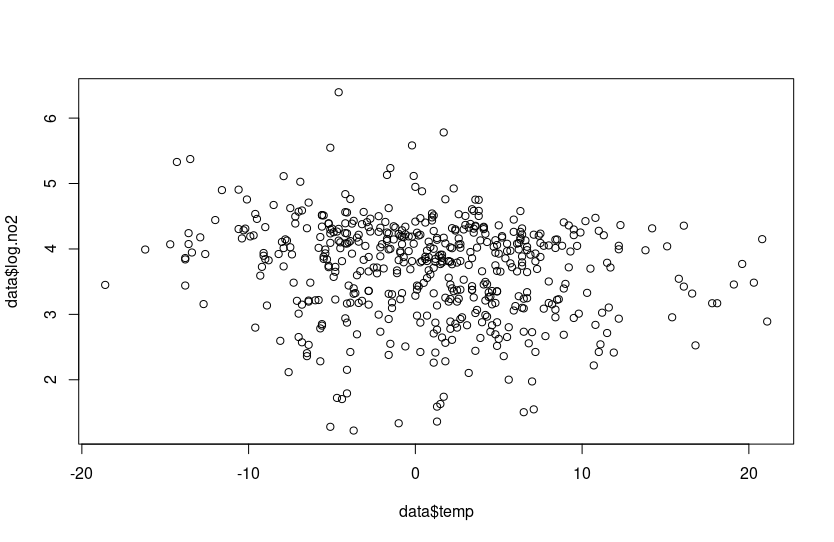
\includegraphics[width=0.7\linewidth]{figures/no2_temp_vs_no2.png}
    \caption{Scatter plot of log NO2 as fuction of temperature.}
    \label{fig:no2_temp_vs_no2}
\end{figure}


\subsubsection*{Hour of day}
In our original model, removing the "hours of day" predictor reduced the $R^2$ score from 0.4615 to 0.4533. However, after our improvements to the model, which now yields $R^2 = 0.4865$, removing the hours of day only reduces this to $R^2 = 0.4841$, suggesting that we are extracting more of the degenerate information from the three other predictors. This can also be seen from the fact that the $|t|$ value of the linear "hours of day" fit fell from $2.926$ to a statistically insignificant value of $1.808$ with our other model improvements. This actually puts it at a non-significant correlation level, and we therefore simply remove "hour of day" as a predictor.


\begin{figure}[h!]
    \centering
    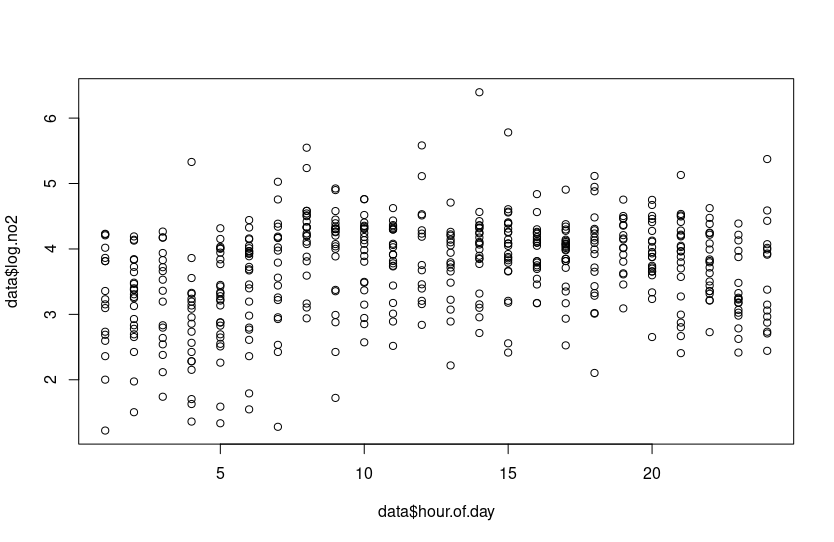
\includegraphics[width=0.7\linewidth]{figures/no2_hour_vs_no2.png}
    \caption{Scatter plot of log NO2 as fuction of hour of day.}
    \label{fig:no2_hour_vs_no2}
\end{figure}


\subsection*{e)}
A lot of this discussion and plots have already been presented in exercise d, but the points are summarize and expand upon here.

Our new final model produce the following results:
\begin{Verbatim}[fontsize=\small]
    Estimate Std. Error t value Pr(>|t|)    
(Intercept)     2.638556   0.086504  30.502  < 2e-16 ***
cuberoot.cars   0.135640   0.007352  18.451  < 2e-16 ***
temp           -0.026862   0.003819  -7.033 6.73e-12 ***
log.wind.speed -0.421724   0.036172 -11.659  < 2e-16 ***

Residual standard error: 0.5391 on 496 degrees of freedom
Multiple R-squared:  0.4872, Adjusted R-squared:  0.4841 
\end{Verbatim}

We see that the intercept of the log.no2 is now actually more than doubled from 1.15 to 2.64. As we don't have any datapoints close to zero, it is natural to have an innacurate intercept.

The cube root of the number of cars is positively correlated with the NO2 level. As both quantities are transformed in different ways, it is difficult to interpret the correlation strength, but of course we at least expected a positive correlation with the number of cars. 

The temperature, which we left unchanged, is negatively correlated with the NO2 level, just as it was in our original model. Whether there is physical justification for this correlation is unknown to me, but the correlation is statistically significant.

The log wind speed is negatively correlated with NO2 levels, just as the linear wind speed was in our original model. Both these correlations make sense, as stronger wind likely helps carry away the NO2 from the polluting cars.

Finally, we removed hours of day as a predictor. Although it actually contributed slightly to the $R^2$-score, it did so at a non-significant level (after our other adjustments). Hour of day is a pretty stupid linear predictor. First of all, the hours of a day are cyclic, with an arbritrary starting point, making it hard to use as a linear (or transformed linear) predictor. Its correlation with the NO2 level, this is entirely through degeneration with other predictors, such as the three others we consider.

\section*{Problem 2}
\subsection*{a)}
Figure \ref{fig:blood_boxplot} shows the distribution of blood pressure values for 12 men (per group) for three different age groups. By eye, all three groups seem to be at least somewhat different, however, the very low number of samples means that this could very well be by chance. Especially the two higher age groups seem pretty overlapping, while the first age group seems more consistently different.
\begin{figure}[h!]
    \centering
    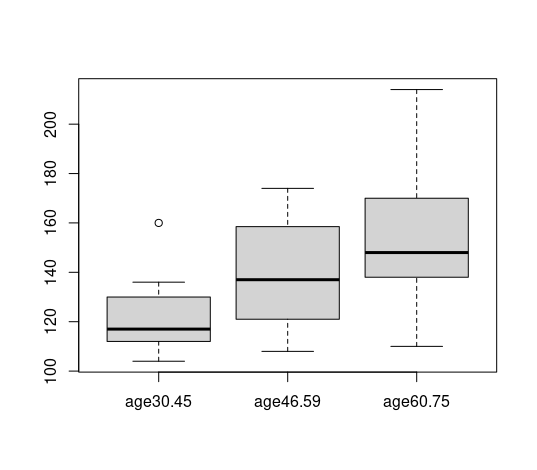
\includegraphics[width=0.7\linewidth]{figures/blood_boxplot.png}
    \caption{Boxplot of blood pressure for three age groups of men, with 12 samples per group.}
    \label{fig:blood_boxplot}
\end{figure}

\subsection*{b)}
A one-way ANOVA test is a test on whether one or more of a series of observables has a different mean than the rest. In other words, the null hypothesis of a one-way ANOVA is that all distribution means are the same, while the alternative hypothesis is that at least one is not. For the test to be valid, we assume that all samples are independently drawn from random distributions with the same standard deviation, and the same mean within a single group.

The result of a one-way ANOVA test gives the following results:
\begin{Verbatim}[fontsize=\small]
    Response: Bloodpr
    Df  Sum Sq Mean Sq F value   Pr(>F)   
agegroup   2  6535.4  3267.7  6.4686 0.004263 **
Residuals 33 16670.2   505.2                   
\end{Verbatim}
The F value of the ANOVA F-test is a quite high 6.4686, which results in a P-value of 0.004263, which is statistically significant at a 95\% level. In other words, we reject the null hypothesis, and conclude that at least one of the means are different. In other words, age \textit{does} have an impact on blood pressure, but we can not from this test alone say \textit{how} age effects blood pressure.


\subsection*{c)}
Since we are only looking at three distinct groups, it would be useful to know which groups are significantly different, and not just that one of them is. We can do this by performing a regression model with categorical predictors. We take the youngest age group as a reference, and look at how much the blood pressure level changes by moving to another group. The mathematical model looks something like
\begin{equation}
    E[\mathrm{blood pressure}_i] = \beta_0 + \beta_1\cdot\mathrm{agegroup2} + \beta_2\cdot\mathrm{agegroup3} + \epsilon_i
\end{equation}
where $\beta_0$ represents the intercept, which is the blood pressure of the lowest age group, while $\mathrm{agegroup2}$ and $\mathrm{agegroup3}$ are binary values representing the two other age groups (in age-ascending order).

Such an analysis gives the following results:
\begin{Verbatim}[fontsize=\small]
    Coefficients:
    Estimate Std. Error t value Pr(>|t|)    
(Intercept)  122.167      6.488  18.829  < 2e-16 ***
agegroup2     16.917      9.176   1.844  0.07423 .  
agegroup3     33.000      9.176   3.596  0.00104 ** 
\end{Verbatim}
A person in the age group 30-45 is expected to have a blood pressure level of $122.167$, which is, on average $16.917$ and $33.000$ higher if belonging to the second and third age groups, respectively. However, the difference of $16.917$ from the default age group is not statistically significant at a $95\%$ level, as its t-value of 1.844 produce a p-value of 0.07423, which is bigger than the threshold of 0.05. The third age group, however, is quite a bit \textit{more} significant than the results we obtained in execise b, and we can confidently conclude that the data supports the fact that the age group 60-75 has a higher blood pressure level than the group 30-45. The fact that we are more confident that these two specific age groups are different, than we were that any group was different in exercise b might seem worrisome. With less conclusive data, this categorical regression test could produce statistical significance, while the ANOVA test insisted the data could not conclude a difference between the groups. Statistics is funny like that.

\clearpage
\section*{Code}
\subsection*{Problem 1a)}
\begin{Verbatim}[fontsize=\footnotesize]
> data = read.delim("../data/no2.txt")
> plot(data$log.cars, data$log.no2)
> summary(data$log.cars)
    Min. 1st Qu.  Median    Mean 3rd Qu.    Max. 
    4.127   6.176   7.425   6.973   7.793   8.349 
> summary(data$log.no2)
    Min. 1st Qu.  Median    Mean 3rd Qu.    Max. 
    1.224   3.214   3.848   3.698   4.217   6.395 
\end{Verbatim}

\subsection*{Problem 1b)}
\begin{Verbatim}[fontsize=\footnotesize]
> fit.cars = lm(log.no2~log.cars, data)
> abline(fit.cars)
\end{Verbatim}

\subsection*{Problem 1c)}
\begin{Verbatim}[fontsize=\footnotesize]
> plot(data$log.cars, fit.cars$residuals)
> hist(fit.cars$residuals, 20)
> plot(fit.cars)
> plot(data$wind.speed, data$log.no2)
> plot(data$temp, data$log.no2)
> plot(data$temp, data$hour.of.day)
\end{Verbatim}

\subsection*{Problem 1d)}
\begin{Verbatim}[fontsize=\footnotesize]

> fit = lm(log.no2~log.cars+temp+wind.speed+hour.of.day, data)
> summary(fit)

Call:
lm(formula = log.no2 ~ log.cars + temp + wind.speed + hour.of.day, 
    data = data)

Residuals:
        Min       1Q   Median       3Q      Max 
-2.24876 -0.32070  0.03084  0.33860  1.96057 

Coefficients:
                Estimate Std. Error t value Pr(>|t|)    
(Intercept)  1.152131   0.175045   6.582 1.19e-10 ***
log.cars     0.456974   0.028411  16.084  < 2e-16 ***
temp        -0.026855   0.003905  -6.877 1.85e-11 ***
wind.speed  -0.149334   0.014076 -10.609  < 2e-16 ***
hour.of.day -0.013025   0.004452  -2.926   0.0036 ** 
---
Signif. codes:  0 ‘***’ 0.001 ‘**’ 0.01 ‘*’ 0.05 ‘.’ 0.1 ‘ ’ 1

Residual standard error: 0.5508 on 495 degrees of freedom
Multiple R-squared:  0.4658,	Adjusted R-squared:  0.4615 
F-statistic: 107.9 on 4 and 495 DF,  p-value: < 2.2e-16



> data$cuberoot.cars <- (exp(data$log.cars))**(1.0/3.0)
> data$log.wind.speed <- log(data$wind.speed)
> fit_new = lm(log.no2~cuberoot.cars+temp+log.wind.speed, data)
> summary(fit_new)

Call:
lm(formula = log.no2 ~ cuberoot.cars + temp + log.wind.speed, 
    data = data)

Residuals:
     Min       1Q   Median       3Q      Max 
-1.99853 -0.33024  0.03479  0.38718  1.84572 

Coefficients:
                Estimate Std. Error t value Pr(>|t|)    
(Intercept)     2.638556   0.086504  30.502  < 2e-16 ***
cuberoot.cars   0.135640   0.007352  18.451  < 2e-16 ***
temp           -0.026862   0.003819  -7.033 6.73e-12 ***
log.wind.speed -0.421724   0.036172 -11.659  < 2e-16 ***
---
Signif. codes:  0 ‘***’ 0.001 ‘**’ 0.01 ‘*’ 0.05 ‘.’ 0.1 ‘ ’ 1

Residual standard error: 0.5391 on 496 degrees of freedom
Multiple R-squared:  0.4872,	Adjusted R-squared:  0.4841 
F-statistic: 157.1 on 3 and 496 DF,  p-value: < 2.2e-16


\end{Verbatim}



\subsection*{Problem 2a)}
\begin{Verbatim}[fontsize=\footnotesize]
> age30.45 <- c(128,104,132,112,136,124,112,118,116,108,160,116)
> age46.59 <- c(120,136,174,166,138,124,160,157,108,110,154,122)
> age60.75 <- c(214,146,138,148,156,110,188,158,182,148,138,136)
> boxplot(age30.45, age46.59, age60.75, names=c("age30.45",
                                    "age46.59","age60.75"))

\end{Verbatim}

\subsection*{Problem 2b)}
\begin{Verbatim}[fontsize=\footnotesize]
> data = read.delim("../data/blood.txt", sep=" ")
> data$agegroup <- factor(data$age)
> fit.aov = aov(Bloodpr~agegroup, data)
> anova(fit.aov)
Analysis of Variance Table

Response: Bloodpr
          Df  Sum Sq Mean Sq F value   Pr(>F)   
agegroup   2  6535.4  3267.7  6.4686 0.004263 **
Residuals 33 16670.2   505.2                    
---
Signif. codes:  0 ‘***’ 0.001 ‘**’ 0.01 ‘*’ 0.05 ‘.’ 0.1 ‘ ’ 1                
\end{Verbatim}

\subsection*{Problem 2c)}
\begin{Verbatim}[fontsize=\footnotesize]
> fit.lm = lm(Bloodpr~agegroup, data)
> summary(fit.lm)

Call:
lm(formula = Bloodpr ~ agegroup, data = data)

Residuals:
    Min      1Q  Median      3Q     Max 
-45.167 -15.583  -5.167  14.104  58.833 

Coefficients:
            Estimate Std. Error t value Pr(>|t|)    
(Intercept)  122.167      6.488  18.829  < 2e-16 ***
agegroup2     16.917      9.176   1.844  0.07423 .  
agegroup3     33.000      9.176   3.596  0.00104 ** 
---
Signif. codes:  0 ‘***’ 0.001 ‘**’ 0.01 ‘*’ 0.05 ‘.’ 0.1 ‘ ’ 1

Residual standard error: 22.48 on 33 degrees of freedom
Multiple R-squared:  0.2816,	Adjusted R-squared:  0.2381 
F-statistic: 6.469 on 2 and 33 DF,  p-value: 0.004263

\end{Verbatim}

\end{document}
